\documentclass{article}
\usepackage[utf8]{inputenc}
\setlength\parindent{0pt}
% \usepackage{nopageno}
\usepackage{amsmath}
\usepackage{amsfonts}
\usepackage{amssymb}
\usepackage{comment}
\usepackage{natbib}
\usepackage{graphicx}
\usepackage{float}
\usepackage{mathtools}
\usepackage{caption}
\usepackage{subcaption}
\usepackage{geometry}
 \geometry{
 a4paper,
 total={170mm,257mm},
 left=30mm,
 right=30mm,
 top=30mm,
 bottom=30mm
}

\setlength{\parskip}{\baselineskip}

\title{Stopping Times for Selecting\\Among Ranked Bernoullis}
\date{}
\author{Patrick Staples}
\begin{document}
\maketitle

\section{Introduction}

We're trying to detect if chunks of text contain some trait (\textit{e.g.}, talk of self-harm). Whether they do or not can be described as a collection of coin flips $y_i \sim \text{Bernoulli}(p_i),\ i=1,...,n$, where $i$ indexes a document, $y_i=1$ if and only if the trait is present in the chunk, and $p_i$ is the probability of $y_i=1$. The task is for a human checker to find all the $\{i: y_i=1\}$, but alas $n$ is so large we can't actually check them all.

The most recent strategy we've discussed is to:
\begin{enumerate}
\item[(1)] rank $n$ chunks from most likely to contain the trait to the least likely,
\item[(2)] verify the most likely ones first, checking in decreasing order of likelihood,
\item[(3)] stop at some point.
\end{enumerate}

If we stop before checking them all, of course we might miss some $y_i=1$ cases. The method proposed here will give an estimate of how many such cases we are likely to have missed for any stopping point.

Assume the ranking above is already done: the ranker tried to re-order the $y_i$s to put $p_i$s in monotonically decreasing order, $p_1 \geq p_2 \geq ... \geq p_n$.

The method we propose makes a \textbf{single key assumption}\footnote{Equation \ref{eq} might not be true. There's no specific reason for the $p_i$ to take this specific form, or even be monotone decreasing. But we have to start somewhere, and I think this assumption will be pretty good if the ranker does its job.}\footnote{Note that Equation \ref{eq} could have just as well been $\text{expit}(a+b\cdot i)$, but then coefficients $a$ and $b$ would rely on $n$, which is inelegant, hence the normalization.}:

\begin{align}
p_i &= \boxed{\text{expit}\left(a + b\cdot \frac{i}{n}\right)}\ ,\text{\ \ \ where\ \ \ expit}(x) := \frac{1}{1+e^{-x}}.\label{eq}
\end{align}

The goal is to check enough chunks such that the expected number of cases among the unchecked chunks, or count of \textit{false negatives} (\text{fn}), is sufficiently low. Formally, the goal is to select $i^*$ satisfying

\begin{align}
\text{fn}(i^*) := \sum_{i=i^*+1}^n \mathbb{E}(y_i) \leq t
\end{align}
for a desired threshold $t$.

\newpage
\section{Methods}

Assume the human checker has already discovered the values $\{y_1, ..., y_{i'}\}$. Is it okay to stop? That is, have we reached $i'=i^*$? If we estimate $a$ and $b$, from Equation/Assumption (\ref{eq}) we immediately have the point estimate:

\begin{align}
\widehat{\text{fn}}(i'; \widehat{a}, \widehat{b}) &= \sum_{i=i'+1}^n \widehat{\mathbb{E}}(y_i) \\
&= \sum_{i=i'+1}^n  \widehat{p_i} \\
&= \sum_{i=i'+1}^n \text{expit}\left(\widehat{a}+\widehat{b}\cdot \frac{i}{n}\right)
\end{align}

Very simply, we can use logistic regression to estimate $a$ and $b$ to accomplish this. Obtain maximum likelihood point estimates (and covariance)\footnote{I'm happy to go into details about how such point estimates and covariance are gotten from maximum likelihood theory, but I imagine you either know it already, or don't but assume the details have been worked out. \newline(They have.)} by modeling:

\begin{align}
\text{logit}(y_i) \sim a + b\cdot \frac{i}{n},\quad i=1, ..., i'
\end{align}

We can even make a predictive distribution for the false negative count, by drawing from:

\begin{align}
\widehat{\text{fn}}(i'; \widehat{a}, \widehat{b}) &\sim \text{fn}(i';\ a', b'), \\
a', b' &\sim \text{Normal}\left((\widehat{a}, \widehat{b}),\ \widehat{\Sigma}(\widehat{a}, \widehat{b})\right).
\end{align}

We're done checking chunks when this distribution shows an acceptable range.\footnote{ \textit{Caveat emptor}: like any predictive distribution, the truth is not guaranteed to be near the average or anything like that, only that the distribution covers the truth, and only approximately so with finite samples. If you run this simulation many times, you'll see this relationship. But simulated coverage is good for $n=1000$ (approximately our case).}

\newpage
\section{Simulation}

Notice that for the $p_i$ to be monotone decreasing, $b$ must be negative. The crisper the ranking, the larger $-b$ will be. Rather than think hard about $a$ directly, I've found it more convenient to only specify a total number of cases $m\in [1, ..., n]$ and use a root solver to find

\begin{align}
a: \frac{1}{n}\sum_{i=1}^n\text{expit}\left(a+b\cdot \frac{i}{n}\right) - \frac{m}{n} = 0.
\end{align}

I've developed simulation code that's easy to modify and play with; I'll introduce the figures they make, and demonstrate a few cases here. Beyond that, playing with the parameters yourself should give you a stronger sense of what's going on.

First, let's plot the ranked $p_i$ values for $n=1000$. In this case, the ranker is only modestly successful: $b:=-10$. The number of cases is $m=100$. Who cares what $a$ turns out to be. The red line shows how many $y_i$ have been checked.\footnote{In the Methods section, this is referred to as $i'$. I've called it $n_{\text{investigated}}$ in the plot for interpretability.}

\begin{figure}[!htb]
    \centering
    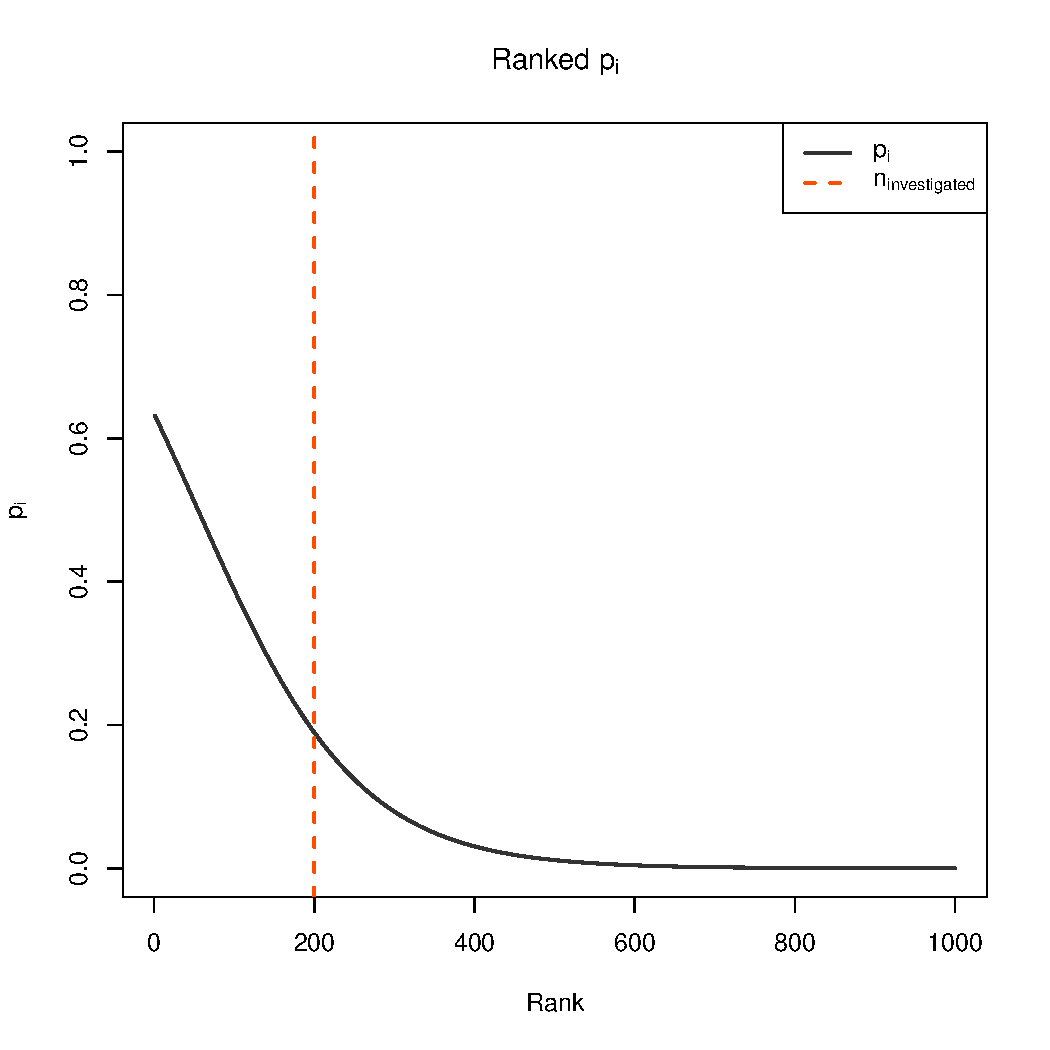
\includegraphics[width=.85\textwidth, trim=0cm 0cm 1cm .5cm, clip]{ranked_rankbad.pdf}
        \label{fig:figure1}
\end{figure}

\newpage
What follows next is a histogram of draws from the predictive distribution of false negatives, $\widehat{\text{fn}}(i'; \widehat{a}, \widehat{b})$. We'd like these numbers to be small enough to stomach. If not low enough, keep checking $y_i$s. I've also put a blue bar showing the true expected number of remaining cases.

Please note that the $y$-axis is log-scaled, and the $x$-axis is not constrained.

\begin{figure}[!htb]
\centering
    \includegraphics[page=2, width=.85\textwidth, trim=0cm 0cm 1cm .5cm, clip]{coverage_rankbad.pdf}
        \label{fig:figure1}
\end{figure}

Are these numbers too high? This is for someone in charge to decide.

The next page shows a progression of three checkpoints for the checker. In this simulation, the ranker is assumed to have had an easier time ($b=-100$).
\begin{itemize}
\item The first row shows a clearly too-early stopping point ($i'=m/2=50$); the resulting false negatives distribution shows abysmally high mean and variance.
\item The middle row shows the situation when the checker notices that the cases currently being checked are 50/50 hit or miss (in stark contrast to earlier checks)\footnote{If Equation \ref{eq} this occurs precisely when $i'=m$.}. This actually looks like an acceptable place to stop!
\item The final row is overkill: they haven't seen a case in a while, they just wanted to be sure. The resulting false negative distribution agrees: the expected number of remaining cases is a strong zero. Not one, zero.
\end{itemize}
\newpage
\begin{figure}[!htb]
    \centering
    \begin{subfigure}{0.45\textwidth}
        \centering
        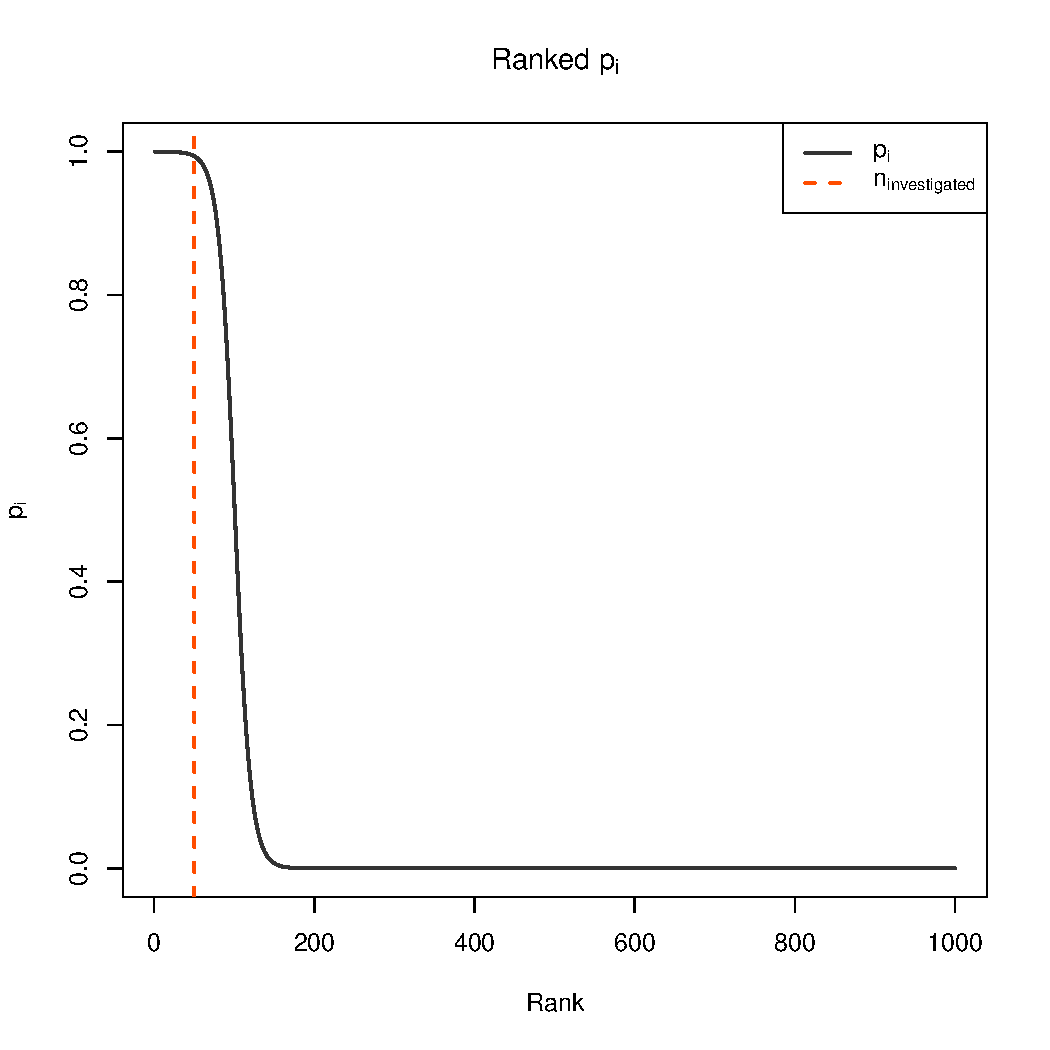
\includegraphics[width=\textwidth, trim=1cm 1cm 1cm .5cm, clip]{ranked_notdone.pdf}
    \end{subfigure}
    \hfill
    \begin{subfigure}{0.45\textwidth}
        \centering
        \includegraphics[page=2, width=\textwidth, trim=1cm 1cm 1cm .5cm, clip]{coverage_notdone.pdf}
    \end{subfigure}
    
    \vspace{1em}
    
    \begin{subfigure}{0.45\textwidth}
        \centering
        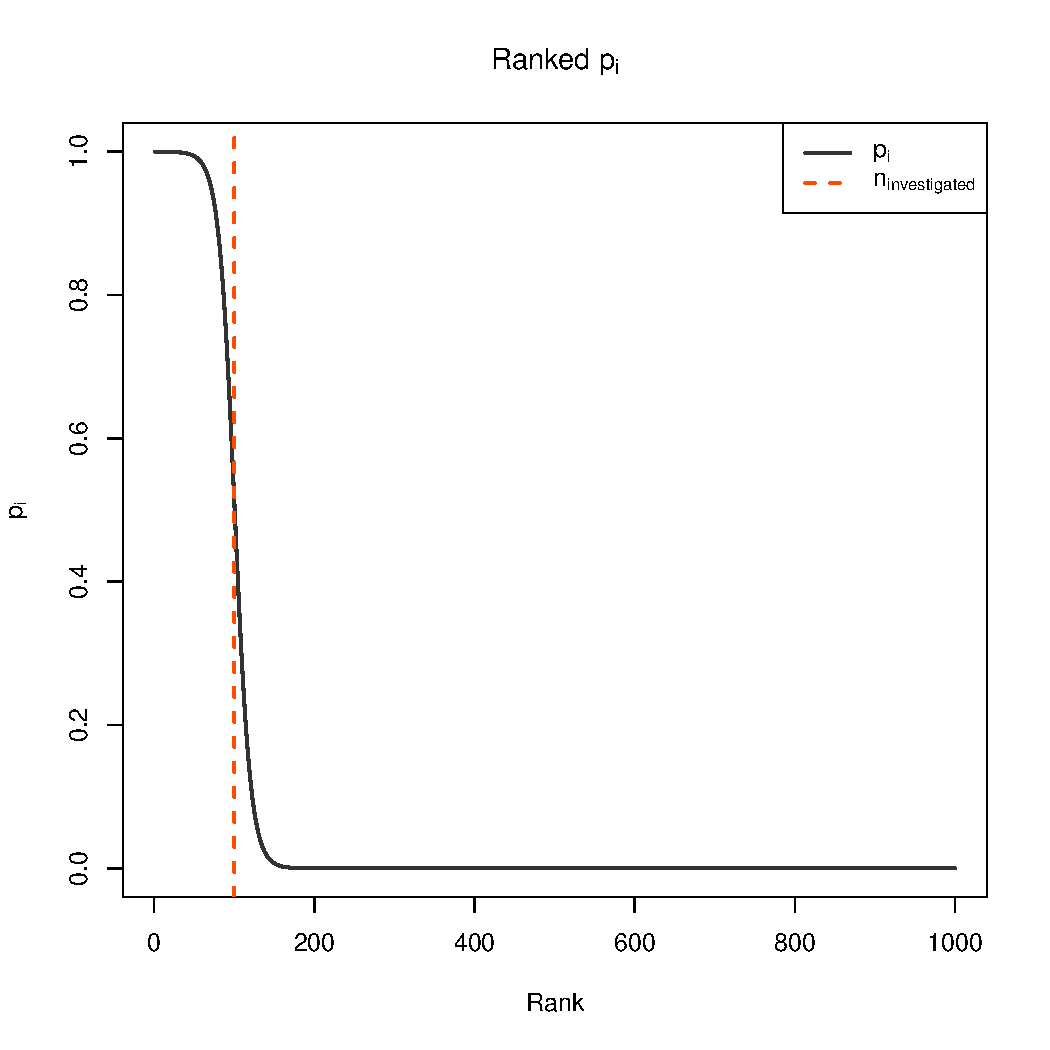
\includegraphics[width=\textwidth, trim=1cm 1cm 1cm .5cm, clip]{ranked_halfhalf.pdf}
    \end{subfigure}
    \hfill
    \begin{subfigure}{0.45\textwidth}
        \centering
        \includegraphics[page=2, width=\textwidth, trim=1cm 1cm 1cm .5cm, clip]{coverage_halfhalf.pdf}
    \end{subfigure}
    
    \vspace{1em}
    
    \begin{subfigure}{0.45\textwidth}
        \centering
        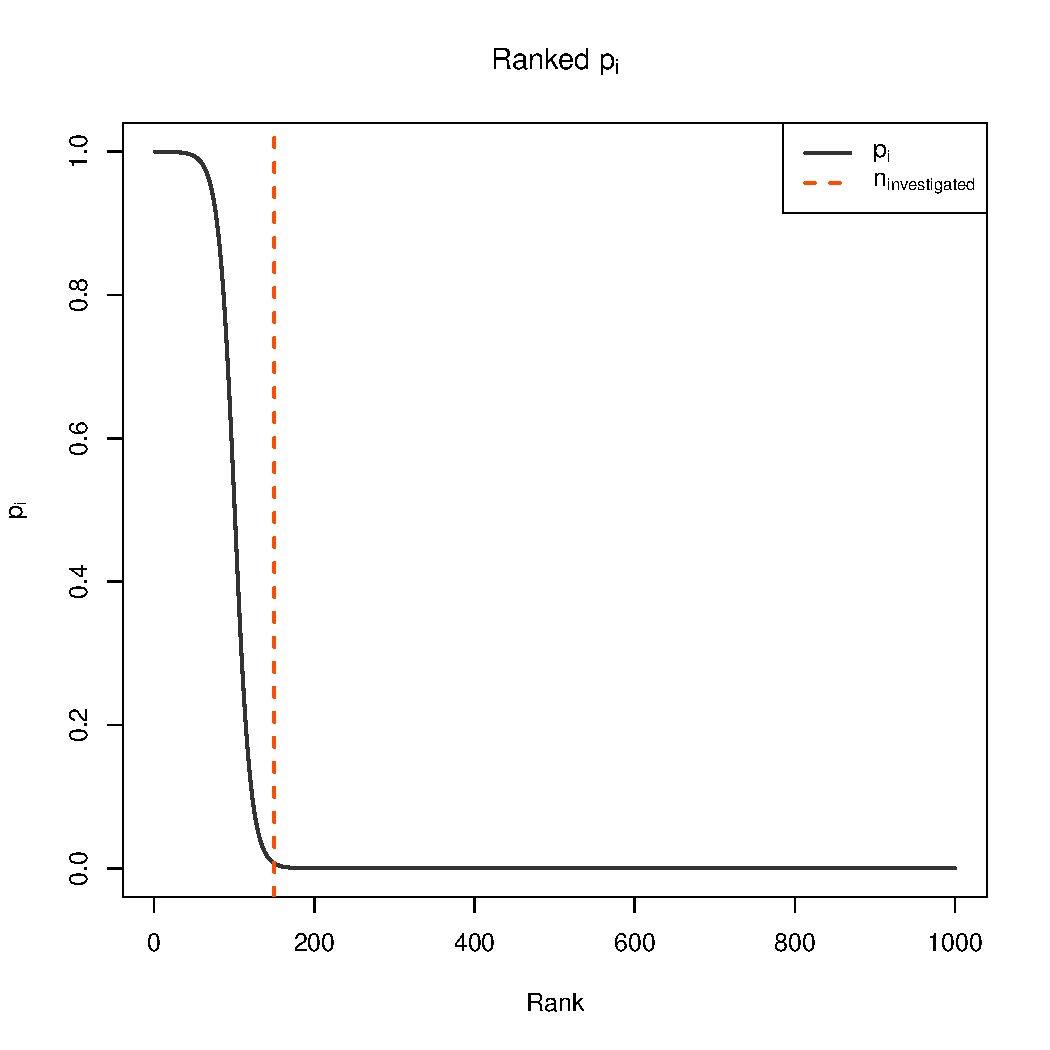
\includegraphics[width=\textwidth, trim=1cm 1cm 1cm .5cm, clip]{ranked_thorough.pdf}
    \end{subfigure}
    \hfill
    \begin{subfigure}{0.45\textwidth}
        \centering
        \includegraphics[page=2, width=\textwidth, trim=1cm 1cm 1cm .5cm, clip]{coverage_thorough.pdf}
    \end{subfigure}
    \label{fig:figures}
\end{figure}

\newpage
\section{\texttt{R} Code}
\begin{verbatim}
library(mvtnorm)

# ### set important params
n = 1000              # total chunks
n_investigated = 100  # how many have been checked
m = 100               # count of true cases
b = -100              # ranker quality (more negative is better quality)

# ### params / data that follow or aren't key for user to specify
B = 100000            # samples from estimated false negative distribution
x = seq(0, 1, length.out=n)
f = function(a) mean(expit(a + b * x)) - m/n
a = uniroot(f, lower=-20, upper=1000)$root
p = expit(a + b * x)  # ranked probabilities
y = rbinom(n, 1, p)   # actual sampled data

# ### plot true ranked probabilities
plot(p, type="l", ylim=c(0, 1), xlab="Rank", main=expression(paste("Ranked ", p[i])),
     ylab=expression(p[i]), lwd=2, col=rgb(.2, .2, .2))
abline(v=n_investigated, lwd=2, col=red, lty=2)
legend("topright", c(expression(p[i]), expression(n[investigated])),
       lwd=2, col=c(rgb(.2, .2, .2), red), lty=c(1, 2))

# ### estimate ranks from data so far
# note: because they're ranked, earlier observations are more likely to be 1s than 0s.
# for better estimation properties, I weight later observations more heavily.
weights = round(sqrt(1:n_investigated))
model <- glm(y[1:n_investigated] ~ x[1:n_investigated], 
             family=binomial(link='logit'), weights=weights)

# ### sample estimated false negatives
draws = rmvnorm(B, mean=model$coefficients, sigma = summary(model)$cov.unscaled)
fn = rep(NA, B)
for(j in 1:B) fn[j] = sum(expit(draws[j, 1] + x[(n_investigated+1):n] * draws[j, 2]))

# ### plot estimated and true false negatives
gray=rgb(0.9, 0.9, 0.9); blue=rgb(0, .4, 1); red=rgb(1, .3, 0)
plt=hist(fn, breaks=100, plot=FALSE)
plt$counts=log10(plt$counts)
plt$counts[plt$counts==-Inf] = 0
y_ticks = 0:4
y_labels <- c("0", expression(10^1), expression(10^2), expression(10^3), expression(10^4))

plot(plt, yaxt="n", col=gray,
     xlab="Estimated Cases Missed by Human", ylab="Simulated Counts")
axis(side = 2, at = y_ticks, labels = y_labels, las = 1)
abline(v=sum(expit(a + x[(n_investigated+1):n] * b)), col=blue, lwd=5)

legend("topright", legend = c("Simulation", "Truth"), fill = c(gray, NA), 
       lwd = c(NA, 4), col = c("black", blue),
       border = c("black", NA), cex = 0.8)
\end{verbatim}



\end{document}

\title{Improved Power Equation for Small-$p$ Binomials\\Applied to AI/Human Label Mismatches}

\section*{Introduction}

Let's say we're in the situation where we want to be powered to detect differences in a biased coin with very low $p := \text{Prob}(\text{heads})$. Specifically, in our case we want to distinguish between a null $H_0: p_0 := c\cdot p_A$, against a (slightly higher but still rare) alternative $p_A$ and $c \in [0,\ 1]$. We want to preserve good type I and II coverage, sacrificing the smallest possible $n$.

\ \\

\section{Normal Power Calculations}
Let's brush off the basics. Take any old sample $x$. By the vanilla central limit theorem,
\begin{align*}
\frac{\bar{x} - \mu_0}{\sigma_0/\sqrt{n}}  \sim Z\ \big|\ \text{H}_0 \\
\frac{\bar{x} - \mu_A}{\sigma_A/\sqrt{n}}  \sim Z\ \big|\ \text{H}_A
\end{align*}

where $Z$ is distributed standard normal. Rearranging:

\begin{align*}
\bar{x} &\sim \frac{\sigma_0}{\sqrt{n}}Z + \mu_0\ \big|\ \text{H}_0 \\
\bar{x} &\sim \frac{\sigma_A}{\sqrt{n}}Z + \mu_A\ \big|\ \text{H}_A
\end{align*}

Without loss of generality (but is exactly our case), let $\mu_A > \mu_0$. The situation looks like this:

\begin{figure}[H]
    \centering
    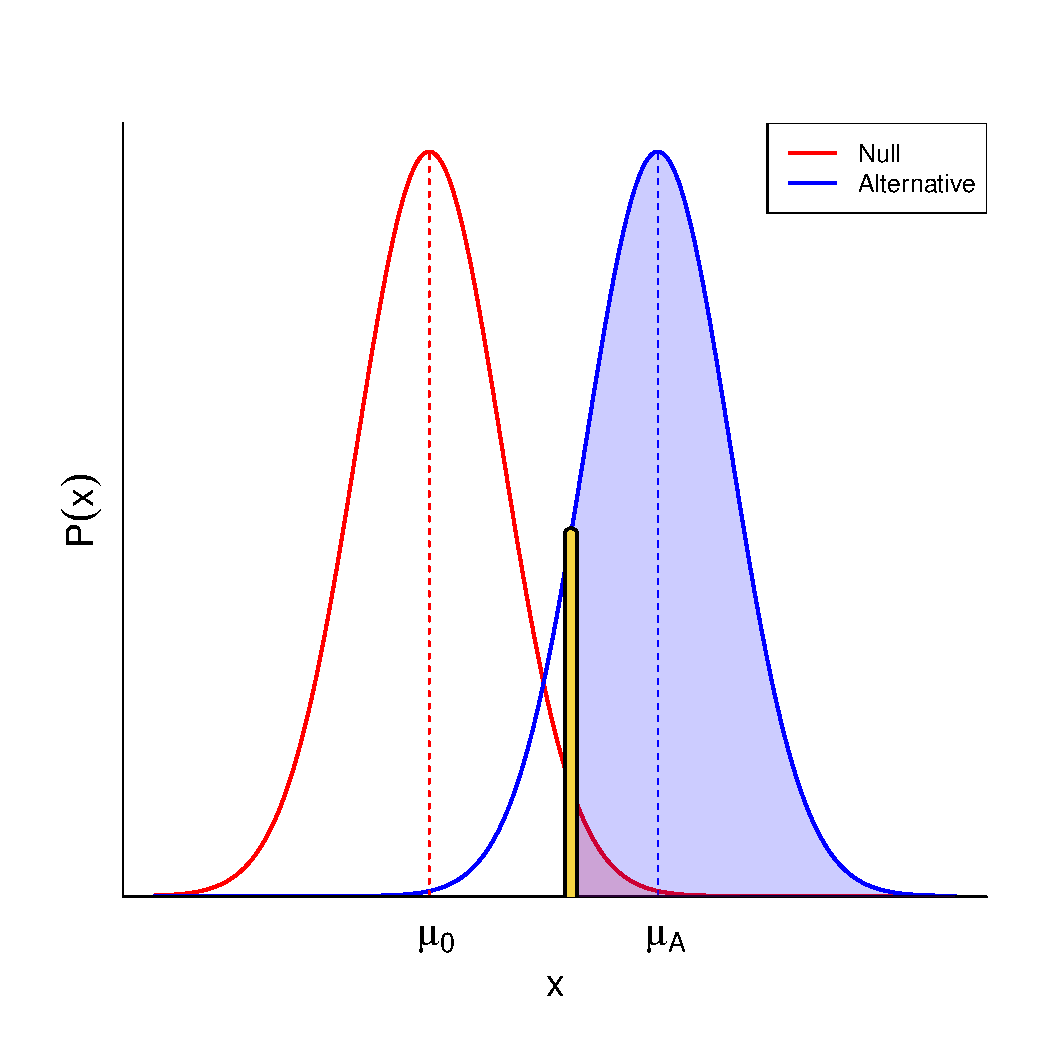
\includegraphics[width=0.9\linewidth]{normals.pdf}
    \caption*{The shaded regions are where the null is rejected under the two hypotheses.}
\end{figure}

We want to find the $x$-value where the yellow line is. Let's call it $Z_c$. We want $Z_c$ to satisfy the two properties:

\begin{align*}
\mathbb{P}(\bar{x} < Z_c \big|\ \text{H}_0) &= 1 - \alpha\\
\mathbb{P}(\bar{x} < Z_c \big|\ \text{H}_A) &= \beta
\end{align*}

These are met respectively when the following two equations hold:

\begin{align*}
Z_c &= \mu_0 + \frac{\sigma_0}{\sqrt{n}}Z_{1 - \alpha} \\
Z_c &= \mu_A + \frac{\sigma_A}{\sqrt{n}}Z_{\beta} = \mu_A - \frac{\sigma_A}{\sqrt{n}}Z_{1 - \beta}
\end{align*}

Because both are equal to $Z_c$, we can drop it and set the two right-hand side expressions as equal:

\begin{align*}
\mu_0 + \frac{\sigma_0}{\sqrt{n}}Z_{1 - \alpha} = \mu_A - \frac{\sigma_A}{\sqrt{n}}Z_{1 - \beta}
\end{align*}

Solving for $n$, we have:

\begin{align*}
\mu_A - \mu_0 &= \frac{1}{\sqrt{n}}\big[\sigma_0Z_{1 - \alpha} + \sigma_AZ_{1 - \beta}\big] \\
\Rightarrow\quad \Aboxed{n &= \left[\frac{\sigma_0Z_{1 - \alpha} + \sigma_AZ_{1 - \beta}}{\mu_A - \mu_0}\right]^2} \\
\end{align*}

\section{The Problem with Small Samples}

Let's now consider the binomial case for a biased coin. Under the Central Limit Theorem,

\begin{align*}
\hat{p} \sim \text{N}\left(0,\ \frac{p(1-p)}{n}\right),\quad n\rightarrow\infty
\end{align*}

We can use this to give a confidence interval for p: $$\widehat{\text{CI}(p)}=\hat{p} \pm q_\alpha\sqrt{\frac{p(1-p)}{n}}$$ where $\alpha$ is the false positive rate and $q_\alpha:=\int_{x=1-\alpha/2}^\infty \mathbb{P}(N(0, 1) = x)$. But for small $n$, this won't be exact because $p\in [0, 1]$, but $\widehat{\text{CI}(p)}$ could be outside $[0, 1]$. Generally, for small $n$, we don't have any guarantee that $100\cdot(1-\alpha)\%$ of the confidence intervals will contain $p$, due to known boundary conditions. This is specifically true in our case: $p$ is near $0$.

\section{Delta Method in our Case}

To recap, for $x_1, ..., x_n \sim X$ with mean $\mu$ and variance $\sigma^2$, the CLT says: $$\bar{x} \sim N(\mu, \sigma^2/n)$$ as $n\rightarrow \infty$. Let's say we want to transform the sample average by appling a function $f$ to it. The CLT still applies! Specifically:

$$f(\bar{x}) \sim N(f(\mu,\sigma^2/n\cdot \left[f'(\mu)\right]^2)$$

This is the \textit{Delta Method}. Here's an idea for how to make a better confidence interval for the proportion: I'll tranform $\hat{p}$ to range between $(-\infty, \infty)$, find a confidence interval for that, then undo the transformation to the resulting lower and upper bounds so that they are also inside $[0, 1]$. Any function $f: [0, 1] \rightarrow (-\infty, \infty)$ will work, but \textbf{I'll pick one}:

\begin{align*}
f(p)&=\text{log}\left(\frac{p}{1-p}\right)
\end{align*}

\ \\

Doing the math, we see that for $f'(p) = \frac{1}{p(1-p)}$, and $\sigma^2 = p(1-p)$. So:

\begin{align*}
f(\hat{p}) &\sim N\left(f(p),\ \frac{1}{p(1-p)n}\right) \\
&=N\left(f(p),\ \frac{f'(p)}{n}\right)
\end{align*}

and the transformed confidence interval is:
\begin{align*}
(\text{lower}, \text{upper}) &= f(\hat{p}) \pm q_{1-\alpha}\sqrt{\frac{f'(\hat{p})}{n}}
\end{align*}

\textit{Aside}: if we wanted to get back a new confidence interval for $\hat{p}$, we can apply $f^{-1}$ to the confidence interval bounds. That is, the new confidence interval is:$$\left(\frac{e^\text{lower}}{1+e^\text{lower}},\ \frac{e^\text{upper}}{1+e^\text{upper}}\right).$$

\newpage{}

Here are some simulations that show that the coverage for this Delta Method are much better than the vanilla CLT:

\begin{figure}[H]
    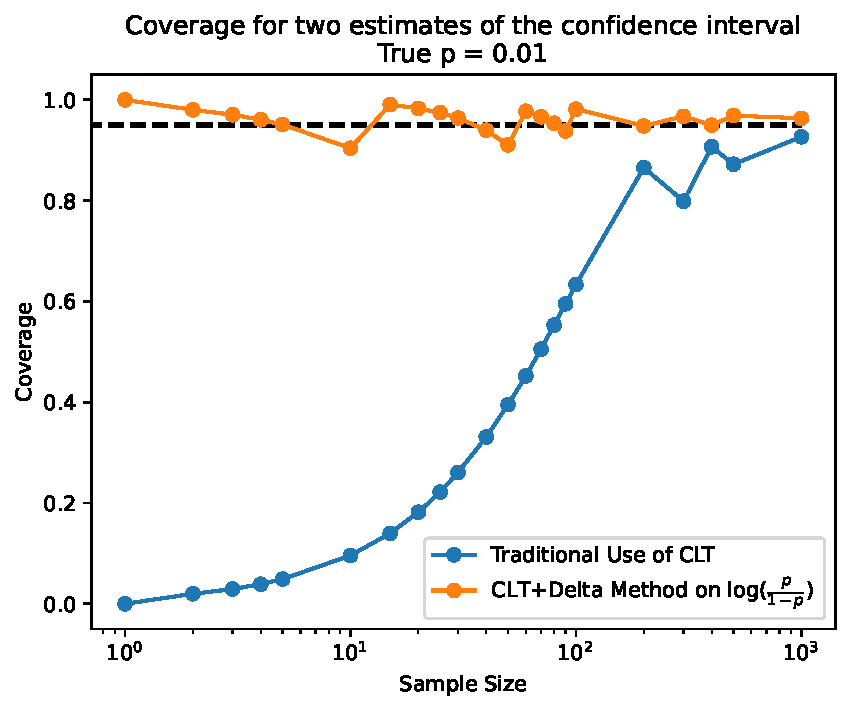
\includegraphics[width=7cm]{plot_0.pdf}
    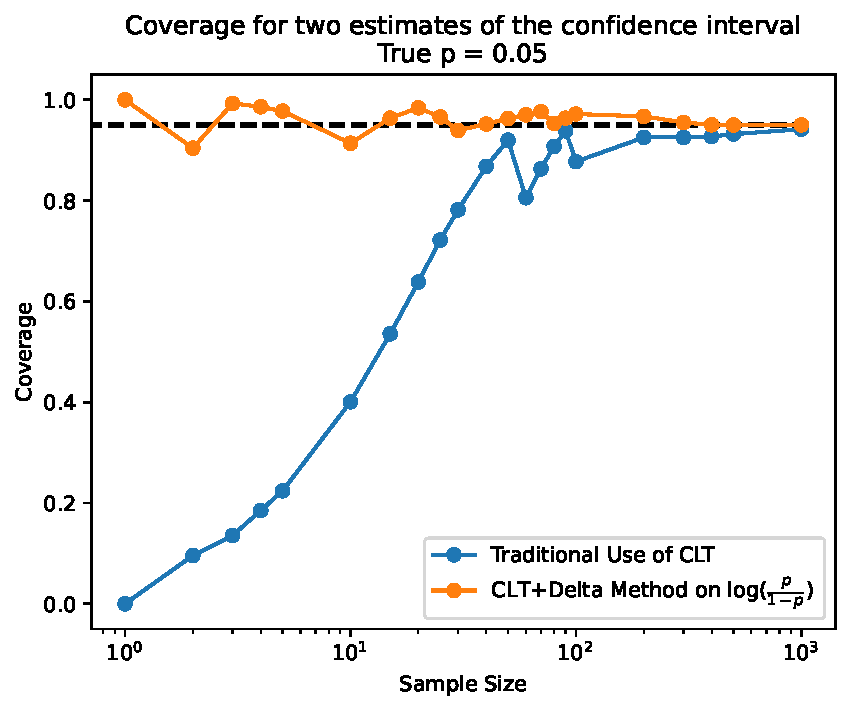
\includegraphics[width=7cm]{plot_1.pdf}
    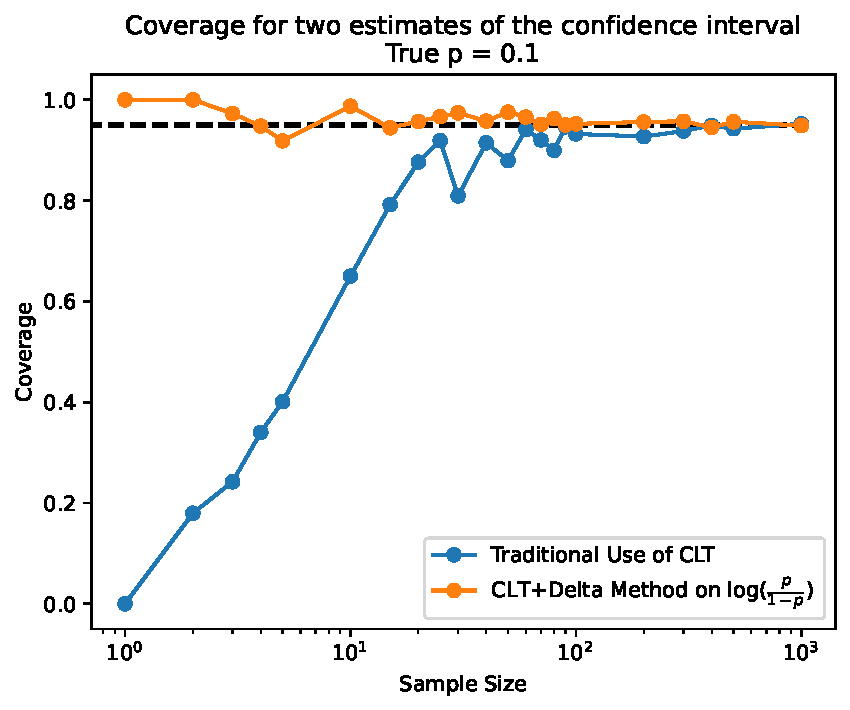
\includegraphics[width=7cm]{plot_2.pdf}
    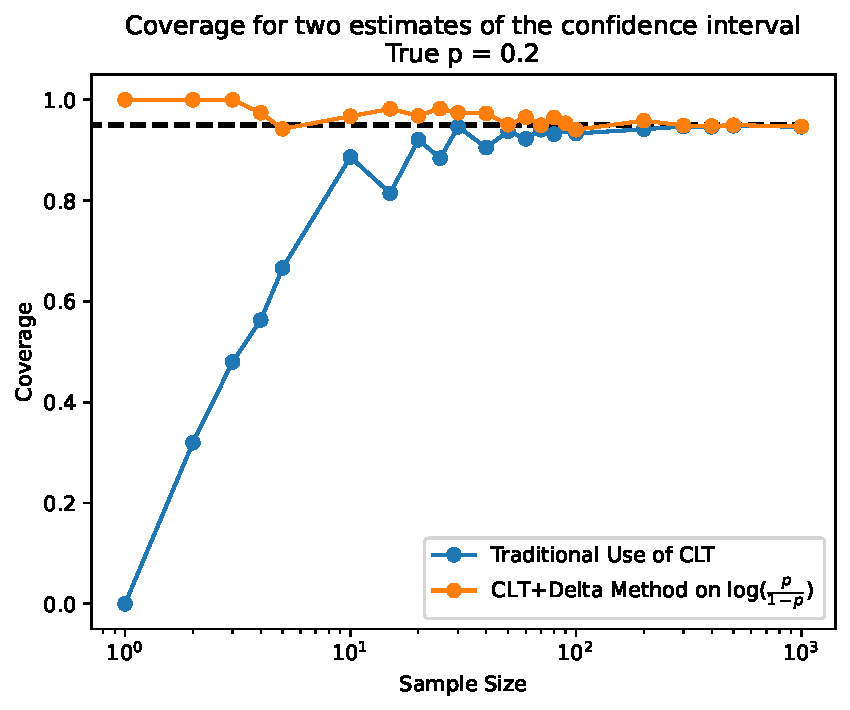
\includegraphics[width=7cm]{plot_3.pdf}
    % 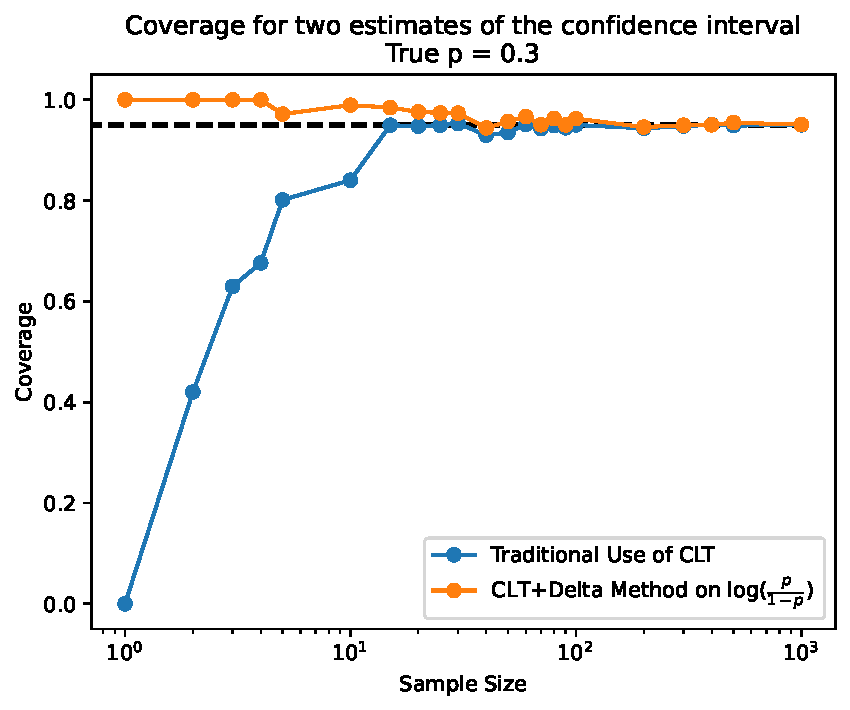
\includegraphics[width=7cm]{plot_4.pdf}
    \caption{Coverage in several boundary conditions.}
    \label{fig:enter-label}
\end{figure}

Obviously this is an improvement: the new method has closer coverage to the asymptotic guarantees.


\section{Modified Power Calculation}

Based on the better empirical coverage shown above, let's re-derive the power calculation based on the normal approximation resulting from the delta transformation. Following the previous development:

\begin{align*}
Z_c &= f(p_0) + q_{1-\alpha}\sqrt{\frac{f'(p_0)}{n}} \text{, and }\\
Z_c &= f(p_A) + q_{\beta}\sqrt{\frac{f'(p_0)}{n}} \\
&= f(p_A) - q_{1-\beta}\sqrt{\frac{f'(p_0)}{n}}
\end{align*}

Setting these two as equal, and rearranging:
\begin{align}
n &= \boxed{\left[\frac{q_{1-\alpha}\sqrt{f'(p_0)}+q_{1-\beta}\sqrt{f'(p_A)}}{f(p_A)-f(p_0)}\right]^2} \label{main_equation}
\end{align}

\section{Example}

In our case we are concerned of a secondary rare event, that two rare-biased coins disagree. Let's say the raw rare even occurs with incidence $i$. If we flip two coins $\text{Ber}(i)$, they will disagree with probability:

\begin{align*}
p := 2i\cdot(1-i)
\end{align*}

Define the \textit{reduction fraction} $c$ as the true fraction of coincidences that actually occur, relative to $p$. That is,
\begin{align*}
p_0 &:=p \\
p_A &=cp
\end{align*}
For clarity in the plots, define the \textit{reduction rate} (in \textit{percent}) as:
\begin{align*}
r := 100\left(1-c\right) (\%)
\end{align*}

Here are the power curves for various incidences $i$ and reductions in incidence $r$:

\begin{figure}[H]
    \centering
    \includegraphics[width=1.2\linewidth]{n to be powered.pdf}
    \caption*{The shaded regions are where the null is rejected under the two hypotheses. This does not use the Delta Method, so coverage is less likely to hold.}
\end{figure}

\begin{figure}[H]
    \centering
    \includegraphics[width=1.2\linewidth]{n to be powered (delta).pdf}
    \caption*{The shaded regions are where the null is rejected under the two hypotheses, in accordance with Equation \ref{main_equation}.}
\end{figure}

\newpage
\section{Code}
\begin{verbatim}
import numpy as np
import scipy.stats as ss
import matplotlib.pyplot as plt

def f(x):
    return np.log(x/(1-x))

def fp(x):
    return 1/(x*(1-x))

alpha = .05
beta = .2
I = np.linspace(.02, .1, 201)
R = np.linspace(10, 95, 101)
def power(i, r):
    pA = 2*i*(1-i)

    c = (1-r/100)*pA
    p0 = c * pA

    q0 = ss.norm(0, 1).ppf(1 - alpha)
    qA = ss.norm(0, 1).ppf(1 - beta)
    num = qA * np.sqrt(fp(pA)) + q0 * np.sqrt(fp(p0)) 
    den = f(pA) - f(p0)
    n = (num/den) ** 2
    return n


pows = [[power(i, r) for i in I] for r in R]
\end{verbatim}

\newpage\begin{verbatim}
# figure
mesh = np.meshgrid(I, R)
plt.figure(figsize=(8, 6))
levels=[50, 75, 100, 125, 150, 200, 300, 400, 500]
contours = plt.contour(*mesh, pows, levels=levels, cmap='coolwarm')
plt.clabel(contours, inline=True, fontsize=10)
plt.colorbar(contours)

plt.title('Sample Size to Reject')
plt.xlabel('True Indicence $i$')
plt.ylabel('Rate of Reduction (%)')

plt.grid(color='gray', linestyle='--', linewidth=0.5)
plt.xticks(np.linspace(0, .1, 11))
plt.yticks(np.linspace(0, 100, 11))

plt.xlim(min(I), max(I))
plt.ylim(min(R), max(R))
plt.savefig('power to reject.pdf', format='pdf', dpi=300, bbox_inches='tight')
plt.show()

\end{verbatim}

%\begin{comment}
This calculator is useful for tests concerning whether the proportions in two groups are different. Suppose the two groups are 'A' and 'B', and we collect a sample from both groups -- i.e. we have two samples. We perform a two-sample test to determine whether the proportion in group A, $p_A$, is different from the proportion in group B, $p_B$. The hypotheses are
$H_0:p_A=p_B$
$H_1:p_A\lt p_B$
.
or
$H_0:p_A=p_B$
$H_1:p_A\gt p_B$
.
where the ratio between the sample sizes of the two groups is
$$\kappa=\frac{n_A}{n_B}$$
Formulas
This calculator uses the following formulas to compute sample size and power, respectively: $$ n_A=\kappa n_B \;\text{ and }\; n_B=\left(\frac{p_A(1-p_A)}{\kappa}+p_B(1-p_B)\right) \left(\frac{z_{1-\alpha}+z_{1-\beta}}{p_A-p_B}\right)^2$$
$$1-\beta=\Phi\left(\frac{|p_A-p_B|}{\sqrt{\frac{p_A(1-p_A)}{n_A}+\frac{p_B(1-p_B)}{n_B}}}-z_{1-\alpha}\right)$$ where

$\kappa=n_A/n_B$ is the matching ratio
$\Phi$ is the standard Normal distribution function
$\Phi^{-1}$ is the standard Normal quantile function
$\alpha$ is Type I error
$\beta$ is Type II error, meaning $1-\beta$ is power

%\end{comment}



